\item
\mbox{}
\begin{center}
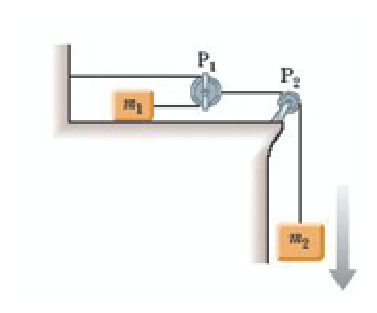
\includegraphics [scale=0.7]{latex/eps/1_5_1_image_1.eps}
%\caption{Gambar katrol}
\end{center}
Sebuah objek bermassa $m_{1}$ berada pada meja horizontal. $m_{1}$ dihubungkan dengan $m_{2}$ oleh katrol tak bermassa $P_{1}$ dan $P_{2}$ seperti pada gambar.\\
a$)$ Cari hubungan percepatan benda 2 dengan percepatan benda 1 ? \\
b$)$ Cari tegangan tali ?\\
c$)$ Cari percepatan benda 1 dan benda 2 dalam $m_{1}$, $m_{2}$, dan $g$ ?
\begin{description}
    \item[Solusi:]
        \mbox{}
\begin{center}
	%\centering
		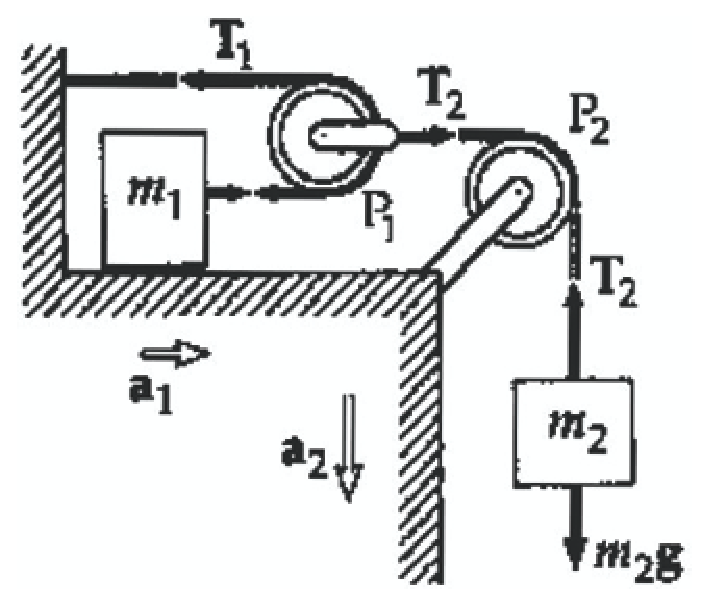
\includegraphics[scale=0.4]{./latex/eps/1_5_1_image_2.eps}
		%\caption{gaya yang bekerja pada katrol}
	%\label{fig:1_5_1_image_2 copy}
%\end{figure}
\end{center}

a$)$lihat gambar 2, katrol $p_{1}$ dan balok $m_{2}$ bergerak dengan percepatan $a_{2}$.
karena balok $m_{1}$ bergerak dengan jarak 2 kali lipat dari jarak katrol $p_{1}$, maka balok $m_{1}$ mempunyai percepatan 2 kali lipat dari percepatan katrol $p_{1}$, maka $a_{1}=2 a_{2}$

b$)$ berdasarkan hukum newton($\sigma f=ma$), maka gaya-gaya yang bekerja pada balok $m_{2}$, $m_{1}$, dan katrol $p_{1}$ berturur-turut adalah
\begin{eqnarray}
	m_{2}g-t_{2}=m_{2}a_{2} \\
	t_{1}=m_{1}a_{1}=2 m_{1}a_{2}\\
	t_{2}-2t_{1}=0
\end{eqnarray}
substitusi $t_{2}$ dari persamaan 3 ke persamaan 1 menjadi $m_{2}g-2t_{1}=m_{2}a_{2} $. persamaan ini dapat dikombinasikan dengan persamaan 2, menjadi
\begin{eqnarray*}
\frac{t_{1}}{m_{1}}\left( 2m_{1}+\frac{m_{2}}{2} \right)=m_{2}g \\
t_{1}=\frac{m_{1}m_{2}}{2 m_{1}+\frac{1}{2}m_{2}}g \quad \mbox{dan} \quad t_{2}=\frac{m_{1}m_{2}}{ m_{1}+\frac{1}{4}m_{2}}g
\end{eqnarray*}

c$)$ setelah mengetahui nilai $t_{1}$ dan $t_{2}$, percepatan dapat dicari dengan menggunakan persamaan 2 
\begin{eqnarray*}
a_{1}=\frac{t_{1}}{m_{1}}=\frac{m_{2} g}{2 m_{1}+\frac{1}{2} m_{2}} \\
a_{2}=\frac{1}{2}a_{1}=\frac{m_{2}g}{4 m_{1+m_{2}}}
\end{eqnarray*}
\end{descriptionn}
